\documentclass{standalone}
\usepackage{tikz}
\usetikzlibrary{patterns}
\usetikzlibrary{positioning}
\usetikzlibrary{patterns, positioning}
\usetikzlibrary{shapes.misc}
\usepackage[outline]{contour}
\contourlength{1.5pt} 


\begin{document}
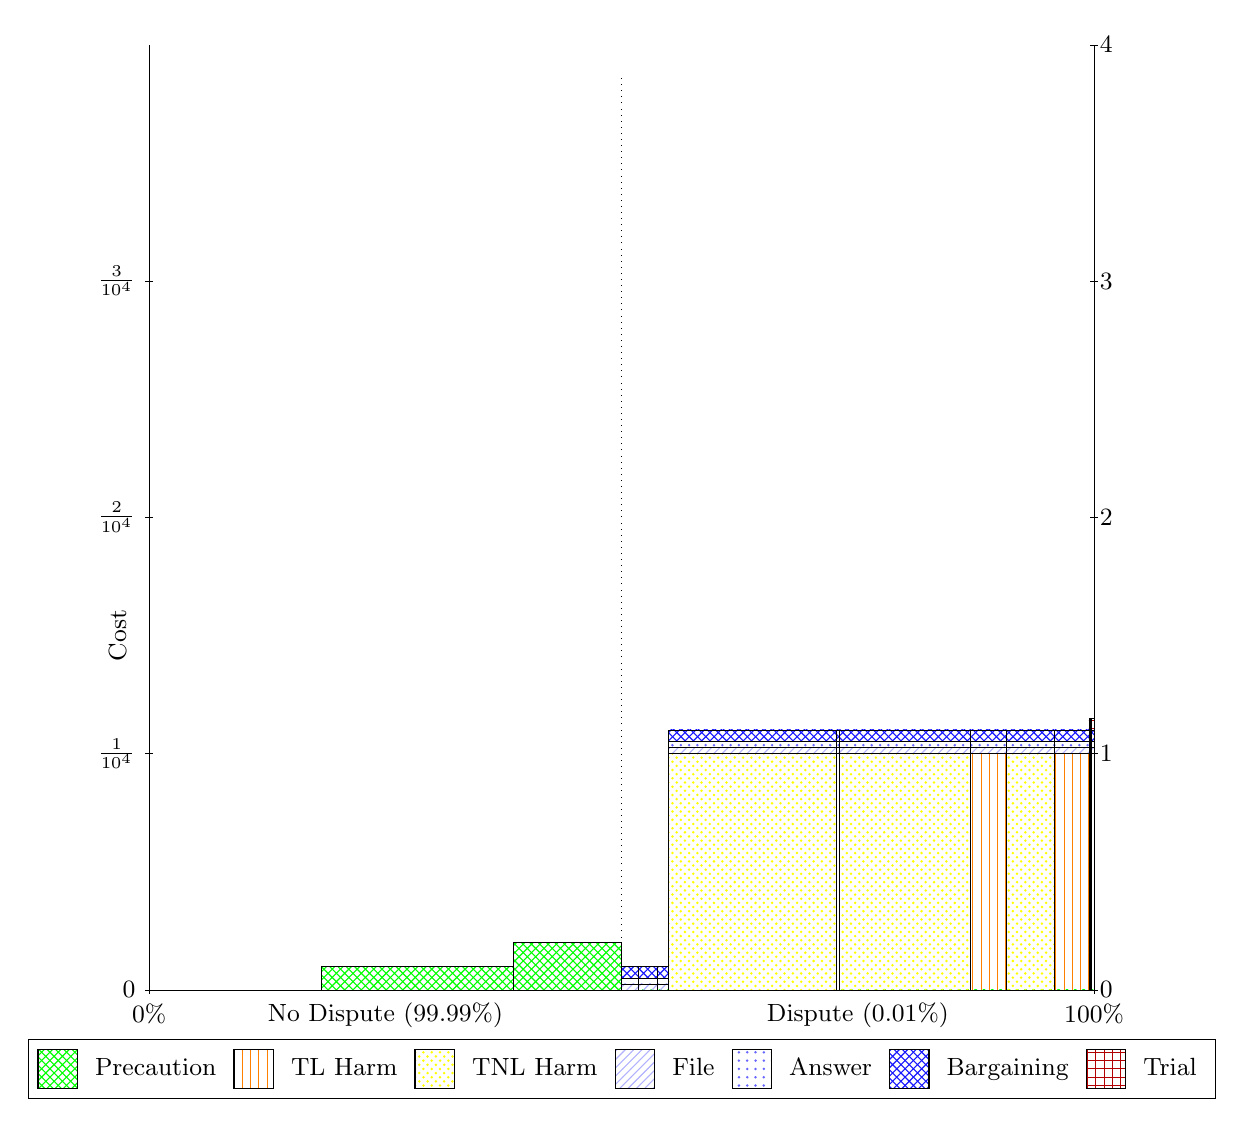
\begin{tikzpicture}
\draw[pattern=crosshatch, pattern color=green,draw=black,very thin] (3.6907,2.5) rectangle (6.1199,2.8001);
\draw[pattern=crosshatch, pattern color=green,draw=black,very thin] (6.1199,2.5) rectangle (7.5,3.1002);
\draw[pattern=north east lines, pattern color=blue!30,draw=black,very thin] (7.5,2.5) rectangle (7.7171,2.575);
\draw[pattern=dots,  pattern color=blue!60,draw=black,very thin] (7.5,2.575) rectangle (7.7171,2.65);
\draw[pattern=crosshatch,      pattern color=blue!90,draw=black,very thin] (7.5,2.65) rectangle (7.7171,2.8);
\draw[pattern=crosshatch, pattern color=green,draw=black,very thin] (7.7171,2.5) rectangle (7.9547,2.5);
\draw[pattern=north east lines, pattern color=blue!30,draw=black,very thin] (7.7171,2.5) rectangle (7.9547,2.575);
\draw[pattern=dots,  pattern color=blue!60,draw=black,very thin] (7.7171,2.575) rectangle (7.9547,2.65);
\draw[pattern=crosshatch,      pattern color=blue!90,draw=black,very thin] (7.7171,2.65) rectangle (7.9547,2.8);
\draw[pattern=crosshatch, pattern color=green,draw=black,very thin] (7.9547,2.5) rectangle (8.0928,2.5001);
\draw[pattern=north east lines, pattern color=blue!30,draw=black,very thin] (7.9547,2.5001) rectangle (8.0928,2.5751);
\draw[pattern=dots,  pattern color=blue!60,draw=black,very thin] (7.9547,2.5751) rectangle (8.0928,2.6501);
\draw[pattern=crosshatch,      pattern color=blue!90,draw=black,very thin] (7.9547,2.6501) rectangle (8.0928,2.8001);
\draw[pattern=crosshatch, pattern color=green,draw=black,very thin] (8.0928,2.5) rectangle (8.0981,2.5);
\draw[pattern=north east lines, pattern color=blue!30,draw=black,very thin] (8.0928,2.5) rectangle (8.0981,2.575);
\draw[pattern=dots,  pattern color=blue!60,draw=black,very thin] (8.0928,2.575) rectangle (8.0981,2.65);
\draw[pattern=crosshatch,      pattern color=blue!90,draw=black,very thin] (8.0928,2.65) rectangle (8.0981,2.8);
\draw[pattern=grid,            pattern color=red!70!black,draw=black,very thin] (8.0928,2.8) rectangle (8.0981,2.95);
\draw[pattern=crosshatch dots, pattern color=yellow,draw=black,very thin] (8.0981,2.5) rectangle (10.219,5.5);
\draw[pattern=north east lines, pattern color=blue!30,draw=black,very thin] (8.0981,5.5) rectangle (10.219,5.575);
\draw[pattern=dots,  pattern color=blue!60,draw=black,very thin] (8.0981,5.575) rectangle (10.219,5.65);
\draw[pattern=crosshatch,      pattern color=blue!90,draw=black,very thin] (8.0981,5.65) rectangle (10.219,5.8);
\draw[pattern=vertical lines, pattern color=orange,draw=black,very thin] (10.219,2.5) rectangle (10.269,5.5);
\draw[pattern=north east lines, pattern color=blue!30,draw=black,very thin] (10.219,5.5) rectangle (10.269,5.575);
\draw[pattern=dots,  pattern color=blue!60,draw=black,very thin] (10.219,5.575) rectangle (10.269,5.65);
\draw[pattern=crosshatch,      pattern color=blue!90,draw=black,very thin] (10.219,5.65) rectangle (10.269,5.8);
\draw[pattern=crosshatch, pattern color=green,draw=black,very thin] (10.269,2.5) rectangle (11.922,2.5);
\draw[pattern=crosshatch dots, pattern color=yellow,draw=black,very thin] (10.269,2.5) rectangle (11.922,5.5);
\draw[pattern=north east lines, pattern color=blue!30,draw=black,very thin] (10.269,5.5) rectangle (11.922,5.575);
\draw[pattern=dots,  pattern color=blue!60,draw=black,very thin] (10.269,5.575) rectangle (11.922,5.65);
\draw[pattern=crosshatch,      pattern color=blue!90,draw=black,very thin] (10.269,5.65) rectangle (11.922,5.8);
\draw[pattern=crosshatch, pattern color=green,draw=black,very thin] (11.922,2.5) rectangle (12.39,2.5);
\draw[pattern=vertical lines, pattern color=orange,draw=black,very thin] (11.922,2.5) rectangle (12.39,5.5);
\draw[pattern=north east lines, pattern color=blue!30,draw=black,very thin] (11.922,5.5) rectangle (12.39,5.575);
\draw[pattern=dots,  pattern color=blue!60,draw=black,very thin] (11.922,5.575) rectangle (12.39,5.65);
\draw[pattern=crosshatch,      pattern color=blue!90,draw=black,very thin] (11.922,5.65) rectangle (12.39,5.8);
\draw[pattern=crosshatch, pattern color=green,draw=black,very thin] (12.39,2.5) rectangle (12.988,2.5001);
\draw[pattern=crosshatch dots, pattern color=yellow,draw=black,very thin] (12.39,2.5001) rectangle (12.988,5.5001);
\draw[pattern=north east lines, pattern color=blue!30,draw=black,very thin] (12.39,5.5001) rectangle (12.988,5.5751);
\draw[pattern=dots,  pattern color=blue!60,draw=black,very thin] (12.39,5.5751) rectangle (12.988,5.6501);
\draw[pattern=crosshatch,      pattern color=blue!90,draw=black,very thin] (12.39,5.6501) rectangle (12.988,5.8001);
\draw[pattern=crosshatch, pattern color=green,draw=black,very thin] (12.988,2.5) rectangle (13.433,2.5001);
\draw[pattern=vertical lines, pattern color=orange,draw=black,very thin] (12.988,2.5001) rectangle (13.433,5.5001);
\draw[pattern=north east lines, pattern color=blue!30,draw=black,very thin] (12.988,5.5001) rectangle (13.433,5.5751);
\draw[pattern=dots,  pattern color=blue!60,draw=black,very thin] (12.988,5.5751) rectangle (13.433,5.6501);
\draw[pattern=crosshatch,      pattern color=blue!90,draw=black,very thin] (12.988,5.6501) rectangle (13.433,5.8001);
\draw[pattern=crosshatch dots, pattern color=yellow,draw=black,very thin] (13.433,2.5) rectangle (13.443,5.5);
\draw[pattern=north east lines, pattern color=blue!30,draw=black,very thin] (13.433,5.5) rectangle (13.443,5.575);
\draw[pattern=dots,  pattern color=blue!60,draw=black,very thin] (13.433,5.575) rectangle (13.443,5.65);
\draw[pattern=crosshatch,      pattern color=blue!90,draw=black,very thin] (13.433,5.65) rectangle (13.443,5.8);
\draw[pattern=grid,            pattern color=red!70!black,draw=black,very thin] (13.433,5.8) rectangle (13.443,5.95);
\draw[pattern=vertical lines, pattern color=orange,draw=black,very thin] (13.443,2.5) rectangle (13.453,5.5);
\draw[pattern=north east lines, pattern color=blue!30,draw=black,very thin] (13.443,5.5) rectangle (13.453,5.575);
\draw[pattern=dots,  pattern color=blue!60,draw=black,very thin] (13.443,5.575) rectangle (13.453,5.65);
\draw[pattern=crosshatch,      pattern color=blue!90,draw=black,very thin] (13.443,5.65) rectangle (13.453,5.8);
\draw[pattern=grid,            pattern color=red!70!black,draw=black,very thin] (13.443,5.8) rectangle (13.453,5.95);
\draw[pattern=crosshatch, pattern color=green,draw=black,very thin] (13.453,2.5) rectangle (13.468,2.5);
\draw[pattern=crosshatch dots, pattern color=yellow,draw=black,very thin] (13.453,2.5) rectangle (13.468,5.5);
\draw[pattern=north east lines, pattern color=blue!30,draw=black,very thin] (13.453,5.5) rectangle (13.468,5.575);
\draw[pattern=dots,  pattern color=blue!60,draw=black,very thin] (13.453,5.575) rectangle (13.468,5.65);
\draw[pattern=crosshatch,      pattern color=blue!90,draw=black,very thin] (13.453,5.65) rectangle (13.468,5.8);
\draw[pattern=grid,            pattern color=red!70!black,draw=black,very thin] (13.453,5.8) rectangle (13.468,5.95);
\draw[pattern=crosshatch, pattern color=green,draw=black,very thin] (13.468,2.5) rectangle (13.5,2.5);
\draw[pattern=vertical lines, pattern color=orange,draw=black,very thin] (13.468,2.5) rectangle (13.5,5.5);
\draw[pattern=north east lines, pattern color=blue!30,draw=black,very thin] (13.468,5.5) rectangle (13.5,5.575);
\draw[pattern=dots,  pattern color=blue!60,draw=black,very thin] (13.468,5.575) rectangle (13.5,5.65);
\draw[pattern=crosshatch,      pattern color=blue!90,draw=black,very thin] (13.468,5.65) rectangle (13.5,5.8);
\draw[pattern=grid,            pattern color=red!70!black,draw=black,very thin] (13.468,5.8) rectangle (13.5,5.95);
\draw[black,very thin] (1.5,2.5) -- (1.5,14.5);
\node[font=\small,rotate=90,text=black, anchor=center] at (1.1, 7.0011) {Cost};
\draw[black,very thin] (1.45,2.5) -- (1.55,2.5);
\node[font=\small,text=black, anchor=east] at (1.45, 2.5) {0};
\draw[black,very thin] (1.45,5.5008) -- (1.55,5.5008);
\node[font=\small,text=black, anchor=east] at (1.45, 5.5008) {$\frac{1}{10^{4}}$};
\draw[black,very thin] (1.45,8.5015) -- (1.55,8.5015);
\node[font=\small,text=black, anchor=east] at (1.45, 8.5015) {$\frac{2}{10^{4}}$};
\draw[black,very thin] (1.45,11.502) -- (1.55,11.502);
\node[font=\small,text=black, anchor=east] at (1.45, 11.502) {$\frac{3}{10^{4}}$};

\draw[black,dotted,very thin] (7.5,2.86) -- (7.5,14.14);
\draw[black,very thin] (13.5,2.5) -- (13.5,14.5);
\draw[black,very thin] (13.45,2.5) -- (13.55,2.5);
\node[font=\small,text=black, anchor=west] at (13.45, 2.5) {0};
\draw[black,very thin] (13.45,5.5) -- (13.55,5.5);
\node[font=\small,text=black, anchor=west] at (13.45, 5.5) {1};
\draw[black,very thin] (13.45,8.5) -- (13.55,8.5);
\node[font=\small,text=black, anchor=west] at (13.45, 8.5) {2};
\draw[black,very thin] (13.45,11.5) -- (13.55,11.5);
\node[font=\small,text=black, anchor=west] at (13.45, 11.5) {3};
\draw[black,very thin] (13.45,14.5) -- (13.55,14.5);
\node[font=\small,text=black, anchor=west] at (13.45, 14.5) {4};

\draw[black,very thin] (1.5,2.5) -- (13.5,2.5);
\draw[black,very thin] (1.5,2.45) -- (1.5,2.55);
\node[font=\small,text=black, anchor=north] at (1.5, 2.45) {0\%};
\draw[black,very thin] (13.5,2.45) -- (13.5,2.55);
\node[font=\small,text=black, anchor=north] at (13.5, 2.45) {100\%};

\node[font=\small,text=black,anchor=south] at (4.5, 1.9) {No\ Dispute\ (99.99\%)};
\node[font=\small,text=black,anchor=south] at (10.5, 1.9) {Dispute\ (0.01\%)};
\draw (7.5,2.5) node (B) {};
\begin{scope}[align=center]
\matrix[scale=0.5,draw=black,below=0.5cm of B,nodes={draw},column sep=0.1cm]{
\node[rectangle,draw,minimum width=0.5cm,minimum height=0.5cm,pattern=crosshatch, pattern color=green]{}; & \node[draw=none,font=\small,text=black]{Precaution}; &
\node[rectangle,draw,minimum width=0.5cm,minimum height=0.5cm,pattern=vertical lines, pattern color=orange]{}; & \node[draw=none,font=\small,text=black]{TL Harm}; &
\node[rectangle,draw,minimum width=0.5cm,minimum height=0.5cm,pattern=crosshatch dots, pattern color=yellow]{}; & \node[draw=none,font=\small,text=black]{TNL Harm}; &
\node[rectangle,draw,minimum width=0.5cm,minimum height=0.5cm,pattern=north east lines, pattern color=blue!30]{}; & \node[draw=none,font=\small,text=black]{File}; &
\node[rectangle,draw,minimum width=0.5cm,minimum height=0.5cm,pattern=dots,  pattern color=blue!60]{}; & \node[draw=none,font=\small,text=black]{Answer}; &
\node[rectangle,draw,minimum width=0.5cm,minimum height=0.5cm,pattern=crosshatch,      pattern color=blue!90]{}; & \node[draw=none,font=\small,text=black]{Bargaining}; &
\node[rectangle,draw,minimum width=0.5cm,minimum height=0.5cm,pattern=grid,            pattern color=red!70!black]{}; & \node[draw=none,font=\small,text=black]{Trial}; \\\\
};\end{scope}

\end{tikzpicture}
\end{document}